\documentclass[a4paper,12pt]{article}
%\usepackage{fullpage}
%\usepackage{pdfpages}

\usepackage{geometry}
 \geometry{
 a4paper,
 total={170mm,257mm},
 left=20mm,
 top=20mm,
 }

\usepackage{color}
\usepackage{amsmath,graphicx,makeidx}
\usepackage{lscape}
\usepackage{fancyhdr}
\addtolength{\headheight}{1.5cm} % make more space for the header
\pagestyle{fancyplain} % use fancy for all pages except chapter start
\lhead{
\includegraphics[height=1.7cm]{FOSSEE-logo}} % left logo
\rhead{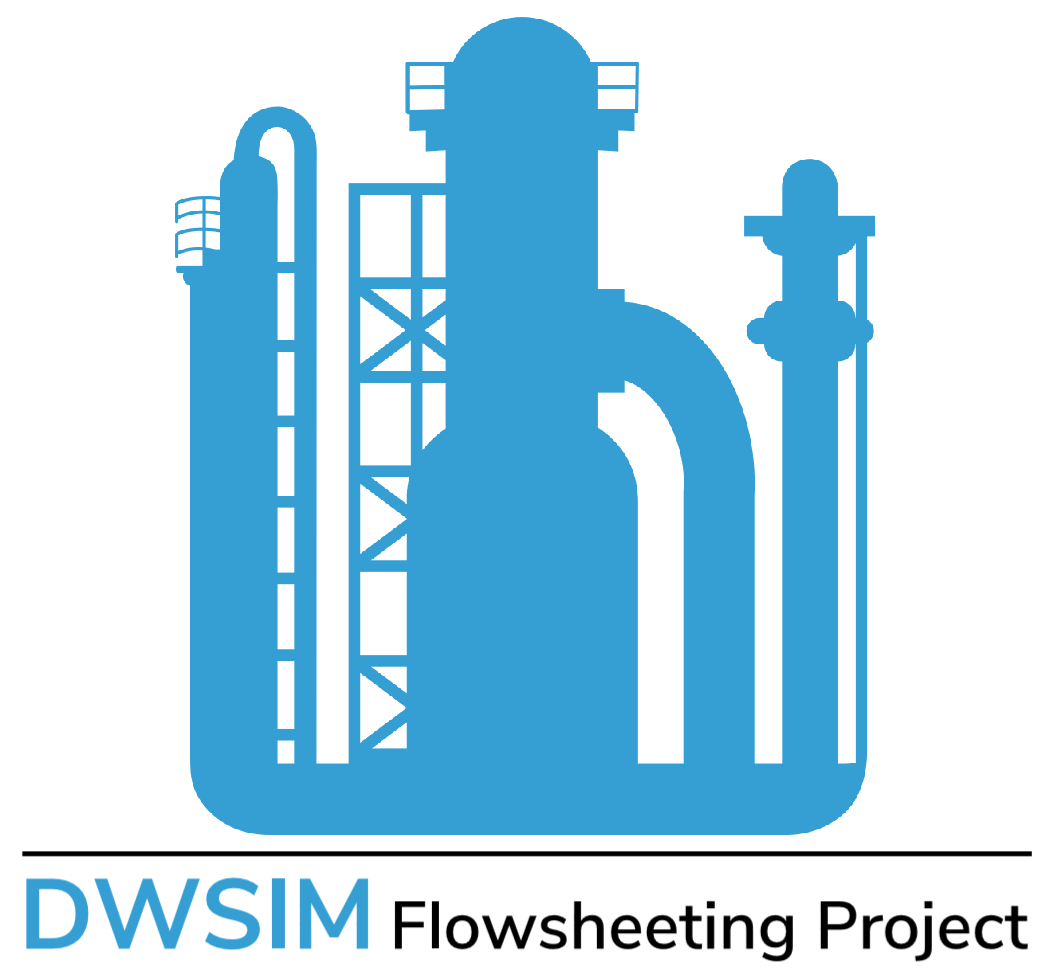
\includegraphics[height=3.5cm]{DWSIM-flowsheeting-project-logo}} % right logo
\renewcommand{\headrulewidth}{0pt} % remove rule below header

\title{Production of Methane from Carbon Monoxide and Hydrogen(using Recycle)}
\author{Pravinkumar Bharat Dalve \\ Indian Institute of Technology Bombay}
\date{}

\begin{document}

\maketitle

\noindent \textbf{Background \& Description:}
\newline A synthesis gas containing $CO$, $H_2$, and a small amount of $CH_4$ with a $CO$ to $H_2$ ratio of 1:2.9 is upgraded to a higher methane content via the reaction

\begin{center}
 $CO + 3H_2 \rightarrow CH_4 + H_20$
\end{center}

The reactor is operated adiabatically with a maximum outlet temperature of 1000$^\circ$F to produce a product stream containing 50\% $CH_4$ and 12\% $CO$. The heat removal rate in the heat exchanger is adjusted to cool the reactor effluent stream to 500$^\circ$F. The separator is operated so as to result in a recycle gas stream containing 1\% $H_2O$ and a pure liquid water stream, both at 100$^\circ$F. The recycle gas stream is sent back to mix with feed and enters the reactor. Both the feed and the product streams are at 200$^\circ$F. The entire system is operated at 100 psia. Separation in DWSIM has been achieved by using compound separator.

\centerline{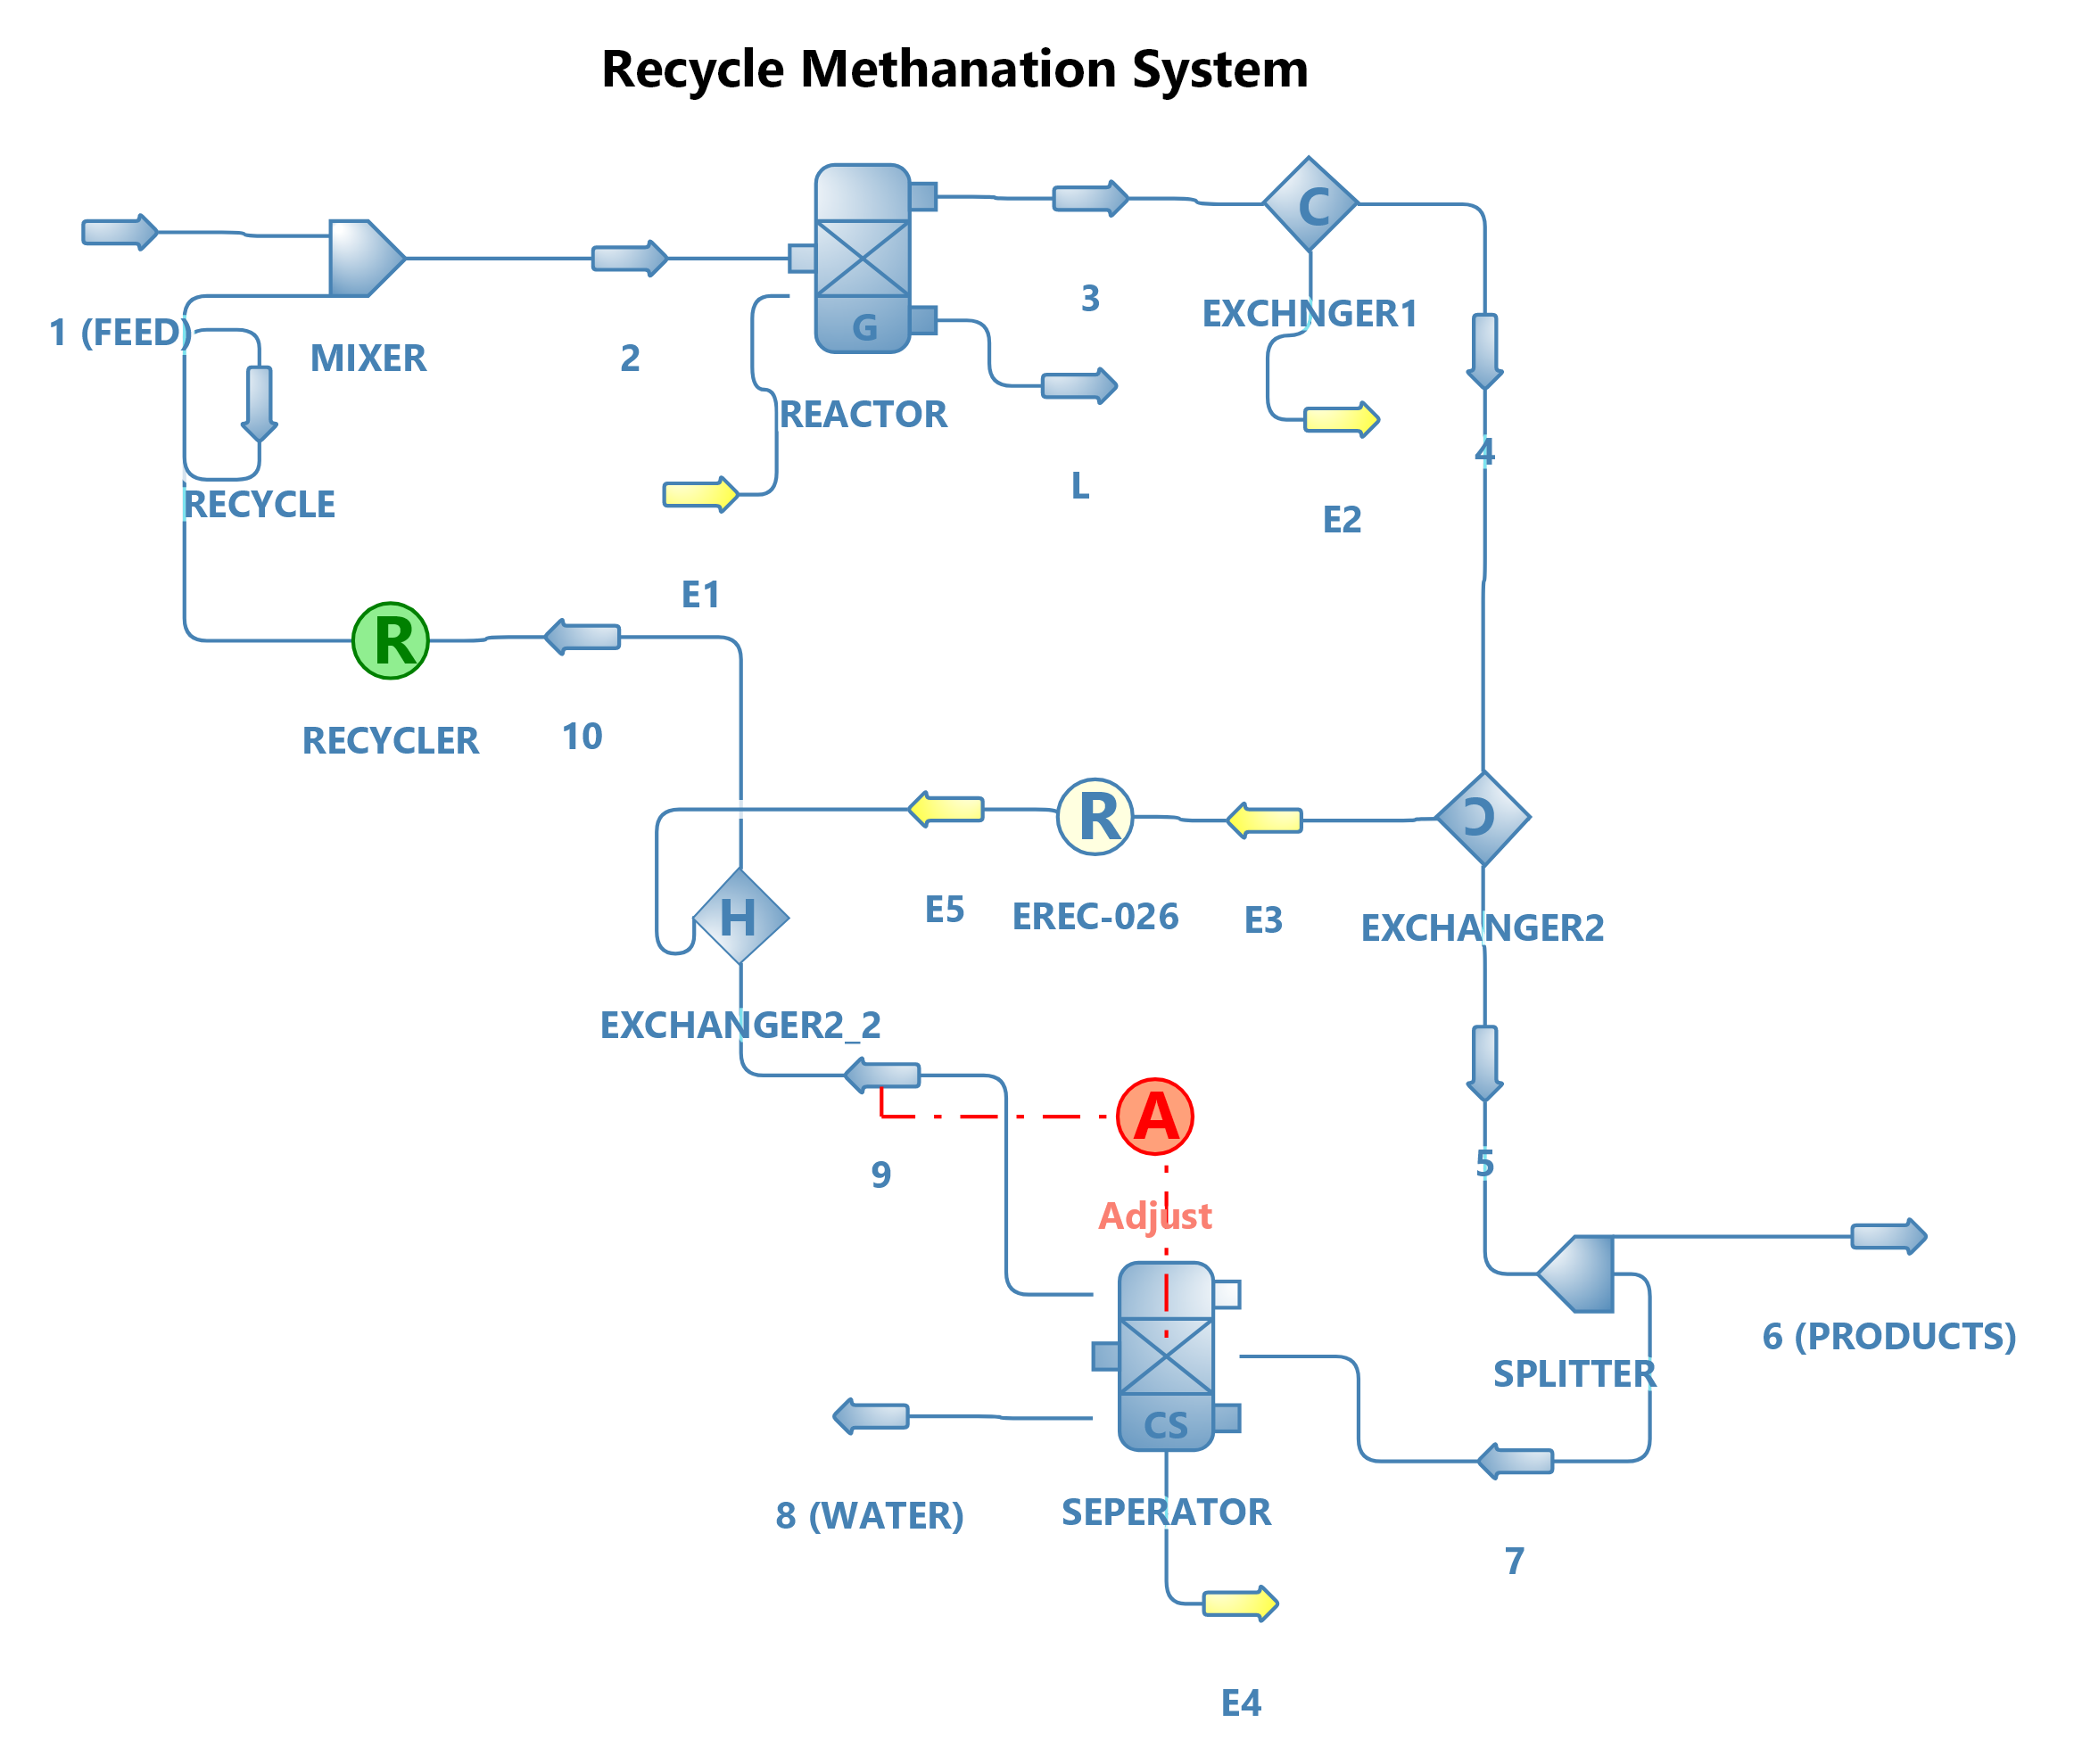
\includegraphics[width=0.9\linewidth]{Meth-Recycle.png}}

\newpage
\noindent \textbf{Results:}
\begin{table}[ht]
\centering
\resizebox{\textwidth}{!}{%
\begin{tabular}{|l|l|l|l|l|l|l|l|}
\hline
Object                                       & RECYCLE   & L        & 9        & 8 (WATER) & 7        & 6 (PRODUCTS) &       \\ \hline
Temperature                                  & 310.92778 & 810.9278 & 366.4833 & 366.4833  & 366.4833 & 366.4833     & K     \\ \hline
Pressure                                     & 92350     & 92350    & 92350    & 92350     & 92350    & 92350        & Pa    \\ \hline
Mass Flow                                    & 1.61607   & 0        & 1.61607  & 0.16206   & 1.77813  & 0.32866      & kg/s  \\ \hline
Molar Flow                                   & 120.59454 & 0        & 120.5945 & 8.99574   & 129.5903 & 23.9527      & mol/s \\ \hline
Molar Fraction (Mixture)  /  Carbon monoxide & 0.11646   & 0        & 0.11646  & 0         & 0.10837  & 0.10837      &       \\ \hline
Molar Fraction (Vapor Phase)  /  Hydrogen    & 0.28911   & 0        & 0.28911  & 0         & 0.26904  & 0.26904      &       \\ \hline
Molar Fraction (Mixture)  /  Methane         & 0.58446   & 0        & 0.58446  & 0         & 0.54389  & 0.54389      &       \\ \hline
Molar Fraction (Mixture)  /  Water           & 0.00997   & 0        & 0.00997  & 1         & 0.07869  & 0.07869      &       \\ \hline \hline
Object                                       & 5         & 4        & 3        & 2         & 10       & 1 (FEED)     &       \\ \hline
Temperature                                  & 366.4833  & 533.15   & 810.9278 & 326.7173  & 310.9278 & 366.4833     & K     \\ \hline
Pressure                                     & 92350     & 92350    & 92350    & 92350     & 92350    & 92350        & Pa    \\ \hline
Mass Flow                                    & 2.10679   & 2.10679  & 2.10679  & 2.10678   & 1.61607  & 0.49015      & kg/s  \\ \hline
Molar Flow                                   & 153.543   & 153.543  & 153.543  & 175.175   & 120.5945 & 54.6161      & mol/s \\ \hline
Molar Fraction (Mixture)  /  Carbon monoxide & 0.10837   & 0.10837  & 0.10837  & 0.15673   & 0.11646  & 0.24618      &       \\ \hline
Molar Fraction (Vapor Phase)  /  Hydrogen    & 0.26904   & 0.26904  & 0.26904  & 0.42105   & 0.28911  & 0.71394      &       \\ \hline
Molar Fraction (Mixture)  /  Methane         & 0.54389   & 0.54389  & 0.54389  & 0.41498   & 0.58446  & 0.03988      &       \\ \hline
Molar Fraction (Mixture)  /  Water           & 0.07869   & 0.07869  & 0.07869  & 0.00723   & 0.00997  & 0            &       \\ \hline
\end{tabular}%
}
\caption{Streamwise Results for Production of Methane Flowsheet}
\end{table}


\end{document}


